\documentclass{report}
\usepackage{hyperref,xcolor,color,titlesec} 
\usepackage{amsmath}
\usepackage{amsfonts}
\usepackage{amssymb}
\usepackage{graphicx}
\hypersetup{
	colorlinks=true,
	linkcolor=blue,  	%setup hyper link styles
	urlcolor=brown
}
\usepackage[none]{hyphenat}%prevents hyphentation
\usepackage{upgreek}
\usepackage{caption}
\usepackage{subcaption}

\titleformat{\chapter}{\normalfont\huge}{\thechapter.}{20pt}{\huge\it} %format chapter/section header styles


%%%%%%%%%%%%%%%%%%%%%%%%%%%%%%%%%%%%%%%%%%%%%%%%%%%%%%%%%%%%%%%%%%%%%%%%%%
%%%%%%SOME FORMATTING MAY NOT WORK IF pdflatex full IS NOT AVAILABLE%%%%%%
%%%%%%%%%%%%%%%%%%%%%%%%%%%%%%%%%%%%%%%%%%%%%%%%%%%%%%%%%%%%%%%%%%%%%%%%%%


\begin{document}

\section{Introduction}

Content Based Image Retrieval  is an application of computer vision 
techniques to a problem known as image retrieval problem. Image retrieval 
problem deals with the searching and retrieval of digital images from 
large databases.\\
\newline
The phrase “content based” means that the process analyzes the contents 
of the image and not the meta-data such as keywords, tags, associated 
descriptions etc. The content in this context may refer to colors, 
shapes, textures, or any other informations that can be derived from the image.\\
\\
In the paper, images were represented by color descriptors. There are 
various color descriptors, but in this paper color histogram, color 
moments and color coherent vector are used as color descriptors. The 
efficiency of these color descriptors to represent visual features of 
images are compared in the paper. 

\section{Motivation}
Content based image retrieval is important because it lacks the drawbacks meta-data based image retrieval has. Searches that rely purely on meta-data are not independent. Rather they depend on annotation quality and completeness. Also to manually annotate images by entering meta-data  or keywords in a large database is time consuming and can have human errors like not capturing the keywords desired to describe a particular image.\\
\\
Content based image retrieval has applications in various important sectors including architectural and engineering design, art collections, crime prevention, geographical information and remote sensing systems, medical diagnosis, military, photograph archive, retail catalogs, nudity-detection filters, face recognition etc. Commercial systems that have been developed based on this include IBM’s QBIC, Virage’s VIR Image Engine, Excalibur’s Image RetrievalWare etc. Also various experimental systems have been and are being developed based on content based image retrieval.

\section{Core Ideas}
CBIR systems manages images by automatically indexing them by summarizing their visual features. A feature can capture some characteristics of images either in a global manner or in a local manner. CBIR systems uses color, textures and shapes as features. Image’s features are extracted by mapping the image pixels to the feature space. Feature spaces are generally represented as feature vectors. Once the features are represented as feature vectors, they can be used to measure similarity between different images.\\
\\
The paper deals with performance of different color descriptors to describe images and based on the description of images the retrieval rate of certain images from the database. For that purpose a fixed color model is selected. The RBG color model is used in this paper. 

\begin{figure}[!h]
\centering
\begin{subfigure}{.5\textwidth}
  \centering
  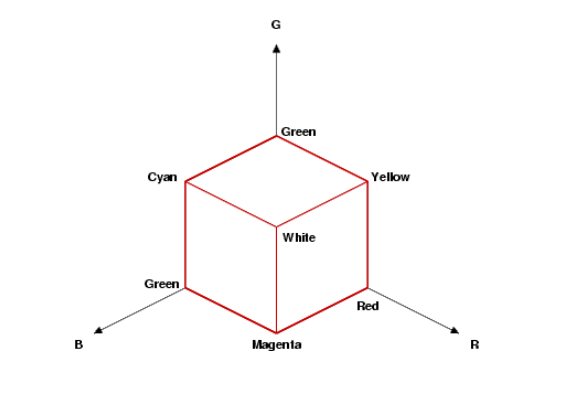
\includegraphics[width=1.1\linewidth]{rgb_ss.png}
  \caption{RGB co-ordinate system}
  \label{fig:RGB1}
\end{subfigure}%
\begin{subfigure}{.5\textwidth}
  \centering
  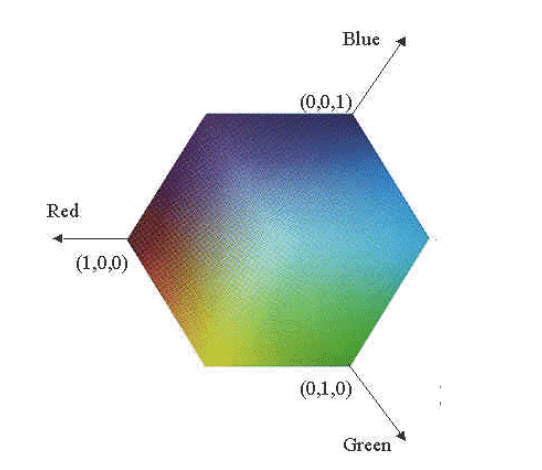
\includegraphics[width=1.1\linewidth]{rgb_sp.png}
  \caption{RGB color}
  \label{fig:RGB2}
\end{subfigure}
\caption{RGB color space}
\label{fig:RGB}
\end{figure}

Color is a very important feature of an image. It doesn’t change whether an image is scaled, translated or rotated. The key components of color feature extraction are color space, color quantification and similarity measurement. A color space is a specific organization of color which allows for reproducible representation of color when combined with physical device profiling.

\subsection{Color Moments}
Color moments are measures that can be used differentiate images based on their features of color. These moments provide a measurement for color similarity between images. These values of similarity can be compared to the values of images in a database for image retrieval. Color moments assume that the distribution of color in an image can be interpreted as a probability distribution. As probability distributions are characterized by a number of unique moments, the color in an image follows a certain probability distribution and the moments of that distribution can be used as features to identify the image based on color.\\
\\
Mean, variance and standard deviation are used as color moments. A color is defined by three or more values. Generally we use hue, saturation and brightness to define a color. In our RGB color space, there are red, blue and green color. For each of the color there are three color moments and so in total nine color moments are computed. \\
\\
Let a image be of size $n\times m$ and $X_{ij}$ be the pixel at $i^{th}$ row and $j^{th}$ column, then,\\
\begin{equation}
mean=\sum_{i=1}^{n}\sum_{j=1}^{m}X_{ij}/(m \times n)\label{eq:1}
\end{equation}
\begin{equation}
variance=\frac{1}{nm}\sum_{i=1}^{n}\sum_{j=1}^{m}(X_{ij}-mean)^{2}\label{eq:2}
\end{equation}
\begin{equation}
stddev=\sqrt{variance}\label{eq:3}
\end{equation}

$INCLUDE\_EXAMPLE$\\ 

\subsection{Color Histogram}
A color histogram is a representation of the distribution of colors in an image. It represents the number of pixels that have colors in each of a fixed list of color ranges that span the image’s color space. The color histogram of a certain image can be built for any kind of color space but in this paper, histogram is built for three-dimensional RGB color space. Color histogram is a statistic that can be viewed as an approximation of an underlying continuous distribution of color values.\\
\\
A color histogram is a graphical representation of the number of pixels in an image. It is a bar graph whose X-axis represents tonal scale and Y-axis represents the number of pixels in an image in a certain area of the tonal scale.\\

\begin{figure}[!h]
\centering
        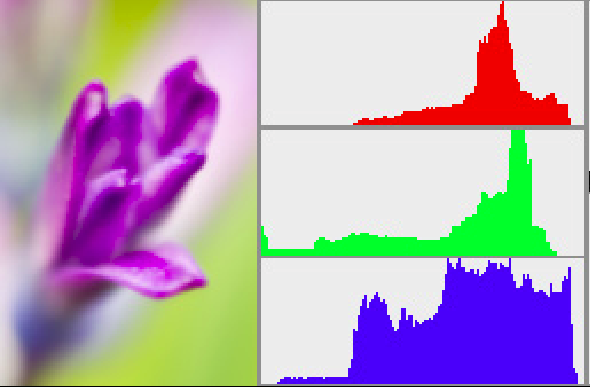
\includegraphics[width=.8\linewidth]{hist_example.png}
    \caption{Histogram of an image}
    \label{fig:verticalcell}
\end{figure}
The color histogram for an image is constructed by counting the number of pixels of each color. There can be a number of elements in the histogram of an image. This number depends on the number of bits in each pixel of an image. If an image has a pixel depth on n bit, then the pixel values of the image will be between $0$  and $2^n-1$. In this case, the histogram will have $2^{n}$ elements.\\
\\
Let, color histogram be $h$. Then it is defined by,\\
\begin{equation}
h_{A,B,C}(a,b,c)=N*Prob(A=a,B=b,C=c)\label{eq:4}
\end{equation}
where A, B and C represent the three color channels (R, G, B) and N is the number of pixels in the image.\\
\\
Computationally, color histogram is made by discretizing the colors within an image and counting the number of pixels of each color. If the data sets are too large, color moments can be computed  by using color histograms.\\
\\ 
\begin{equation}
mean=\sum_{i=0}^{255}i*h(i)/\sum_{i=0}^{255}h(i)\label{eq:5}
\end{equation}
\begin{equation}
variance=\sqrt \frac{\displaystyle \sum_{i=0}^{255}h(i)*(i-mean)^2}{\displaystyle\sum_{i=0}^{255}h(i)}\label{eq:6}
\end{equation}
Here $h=$ histogram of the image\\
\\
In this experiment two techniques of histogram based image retrieval are used. The first one is Global Color Histogram (GCH) and the next one is Local Color Histogram (LCH). In GCH, the whole image is represented by a single histogram. In LCH, the image is divided into blocks of 8x8 and for each of the blocks a histogram is computed.\\
In both cases, the histograms of query image and database’s images are compared and relevant images are retrieved. Let h and g represent two color histograms. Then the euclidean distance between the color histograms $h$ and $g$ can be computed as: 
\begin{equation}
d^2(h,g)=\sum_A\sum_B\sum_C(h(a,b,c)-g(a,b,c))^2\label{eq:7}
\end{equation}
In this case the comparison deals only with identical bins in the respective histograms.

\subsection{Color Coherent Vector}
Color coherent vector is similar to color histogram. Color coherence is the degree to which pixels of some color are members of large similarly colored regions. We refer this regions as coherent regions. Coherent regions are of significant importance in characterizing images. Depending on the size of coherent region, coherent pixels are selected and using those color coherence vector for the images are computed. These CCVs are used to compare the differences and similarities between different images.\\
\\
Color coherent vectors takes the spatial informations of images into count. Color histogram doesn’t take this into count. As a result two or more images can have the same color histogram.\\
\begin{figure}[!h]
\centering
        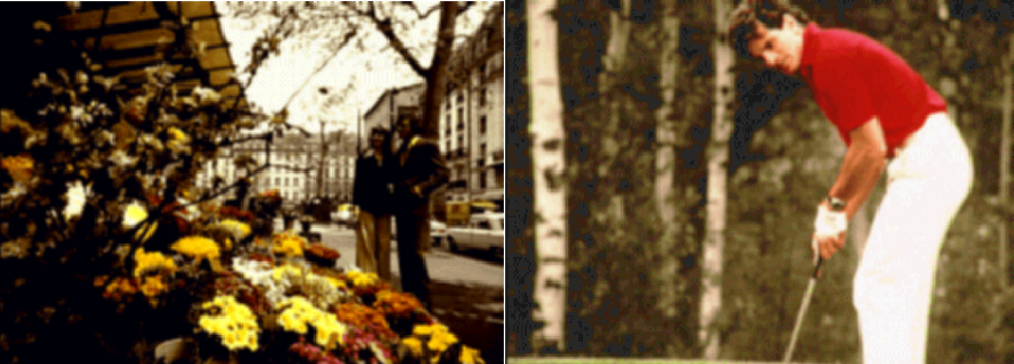
\includegraphics[width=\linewidth]{hist_ccv.png}
    \caption{Two images with similar color histogram}
    \label{fig:similar histogram}
\end{figure}
The images shown in Figure \ref{fig:similar histogram} have similar color histogram although their appearances are clearly different. The color red appears in both images in approximately the same quantities. In left image the red pixels (from the flowers) are widely scattered while in the right image the red pixels (from the golfer’s shirt) form a single coherent region.\\
\\
Our coherence measure classifies pixels as either coherent or incoherent. Coherent pixels are a part of sizable contiguous region while incoherent pixels are not. A color coherent vector represents this classification for each color in the image. CCV’s prevent coherent pixels in one image from matching incoherent pixels in another. This allows fine distinctions that can’t be achieved with color histograms.\\
\\
To classify the pixels within a given color bucket as either coherent or incoherent, some steps are taken. A coherent pixel is part of a large group of pixel of the same color, while an incoherent pixel is not. To determine coherent pixels ‘pixel groups’ are calculated. We determine pixel groups by computing connected components.\\
\\
A connected component $C$ is a maximal set of points such that for any two points $p,p' \in C$, there is a path between $p$ and $p'$. We only compute connected components within a given discretized color bucket.\\
\\
\begin{figure}[!h]
\centering
        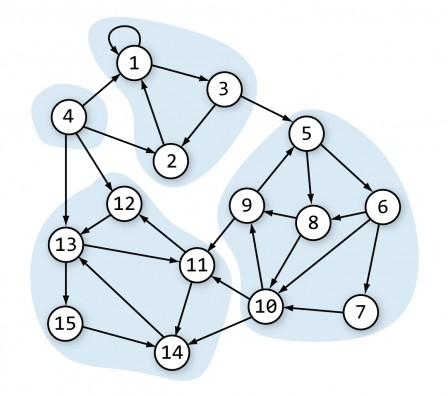
\includegraphics[width=.4\linewidth]{connected.jpg}
    \caption{Connected components}
    \label{fig:connected}
\end{figure}
\\
The connected component can be computed in linear time. When it is completed, each pixel will belong to exactly one connected component. We classify each pixel as coherent or incoherent based on the size of its connected component. A pixel is considered coherent if its connected component’s size exceeds a fixed value $\mathrm{T}$. All other pixels are considered incoherent.\\

\section{Things To Evaluate}
There are eight similarity measurements which can be used to measure the similarities between images. But in this paper, Sum of Squared Differences (SSD) and Sum of Absolute Differences (SAD) are used. These two methods are reported to have the most effectiveness and efficiency. 
\\
\begin{equation}
SSD(f_q,f_t)=\sum_{i=0}^{n-1}(f_q[i]-f_t[i])^2\label{eq:8}
\end{equation}
\begin{equation}
SAD(f_q,f_t)=\sum_{i=0}^{n-1}(f_q[i]-f_t[i])\label{eq:9}
\end{equation}
\\
Here,\\
$f_{q}=$ query feature vector\\
$f_{t}=$ database feature vectors\\
$n=$ the number of features in each vector\\
\\
We used a general purpose database containing 14500 images drawn from different categories to evaluate the effectiveness and efficiency of the selected color descriptors. In the database, the images have dimension of 384X256. We calculated the color features of different images in the database and stored them in a database.\\
\\
The color features are evaluated by means of two ratios: precision and recall. Precision is the ratio of relevant retrieved images to the total retrieved images. Recall is the ratio of relevant retrieved images to the total relevant images in the database.\\
\\
\large
$Precision=\frac{Number \: of\: relevant\: retrived\: images}{Number \: of\: total\: retrived\: images}$\\
\\
$Recall=\frac{Number \: of\: relevant\: retrived\: images}{Number \: of\: total\: relevant\: images \: in \: the\: database}$
\normalfont

\section{Evaluation Process}
Normal images are generally of true color. These images are $24$-bits. So there can a total of $2^{24}$ or $16777216$ color variations. The images both in the database and in the query lists, are quantized to reduce the number of colors from $2^{24}$ to $256$. So the images will be of $8$-bit colors.\\
\begin{figure}[!h]
\centering
\begin{subfigure}{.5\textwidth}
  \centering
  
\includegraphics[width=.9\linewidth]{Truecolor.png}
  \caption{True Color Picture}
  \label{fig:TC}
\end{subfigure}%
\begin{subfigure}{.5\textwidth}
  \centering
  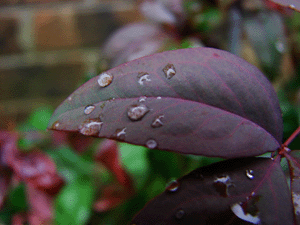
\includegraphics[width=.9\linewidth]{8_bit.png}
  \caption{8-bit Color Picture}
  \label{fig:tb}
\end{subfigure}
\caption{True color \& 8-bit representation of an image}
\label{fig:CC}
\end{figure}


\subsection{Histogram Based Image Retrieval}
$PICTURE\: from\: tikz$\\
\\
First the global/local color histograms for each of the database images are calculated and stored. Then the query image is processed and global/local histogram for the query image is computed. Then using Euclidean distance metrics like //$refer to some equtaiton \#\#1$ the similarities of between the query image and the database images are calculated. A fixed threshold value is taken into account to identify the relevant images.\\
\\
\subsection{Color Moment Based Image Retrieval}
$PICTURE\: of\: tikz$\\
\\
The visual features of an image is extracted using the //equationss…. Color moments are also computed using the histogram computed in the previous process. These are calculated for database’s images and stored. Then query image’s mean, standard deviation are calculated. After that these are compared with the same types in the database image. A threshold value is fixed which depends on the difference between mean and standard deviation of query image and database images. The relevant images are ranked using it.\\
\subsection{Color Coherent Vector Based Image Retrieval}
$PICTURE\: of\: tikz$\\
\\
First for all the images in the database, the pixels in the images are categorized as coherent or incoherent by computing connected component. Then we use a  color coherent vector to represent this classification for each of the colors. We replace the  pixel values with the average value in a small neighborhood. As a result the image is slightly blurred. This can be done using gaussian filter. We descretize the color space so that only R,G and B colors are present in the image. Then color coherent vector is computed for the database images and query images. We retrieve the relevant images by comparing the similarity between query vector and database’s image vectors.\\
\\
We used combination of different color features and retrieving images based on it.\\

\section{Results}
We used the previously mentioned database. The database has categories like  Africans and villages, Beaches, Buildings, Buses, Dinosaurs, Elephants, Flowers, Horses, Mountains and glaciers, Food, Faces, Objects, Drawings, Textures and Natural scenes. Five images of each of the types are used as query images for the retrieval purpose. All these images quality are different. Some have uniform color distribution, some have non-uniform color distribution and others have widely scattered colors. The tables below shows parts of our result.\\
$TABLE1$\\
$TABLE2$\\
\\
We can see the precision and recall of the color descriptors in the tables. The color moments gave better result when the color distribution is of average level. Color histogram gives better result in case of uniform color distribution images. And for widely scattered colors Color Coherent Vector gives the best result. But the combination of different color descriptors produce remarkable results among all.\\
\\
\section{Conclusion}
In the paper, comparison of three color feature for image retrieval is presented. The analysis and the data collection process that are presented in the paper are quite agreeable. These data can be used to further test and analyze the new systems built on the similar principles. As with time new methods of image retrieval are being discovered, these results as well as the process of achieving these results can come to help to further facilitate research in related areas.


\end{document}